% Research Paper for GECCO 2015
% by Nic McPhee, Kirbie Dramdahl, and David Donatucci

\documentclass{sig-alternate}

\usepackage{graphicx}
\usepackage{algorithm}
\usepackage{algpseudocode}
\usepackage{url}
\sloppy

\newcommand{\citep}[1]{\cite{#1}}

\DeclareGraphicsRule{.tif}{png}{.png}{`convert #1 `dirname #1`/`basename #1 .tif`.png}

\begin{document}

\setcopyright{acmlicensed}
\conferenceinfo{GECCO '15,}{July 11 - 15, 2015, Madrid, Spain}
\isbn{978-1-4503-3472-3/15/07}\acmPrice{\$15.00}
\doi{http://dx.doi.org/10.1145/2739480.2754778}

%\CopyrightYear{2015}
%\crdata{TBA}
\clubpenalty=10000
\widowpenalty = 10000
    
\title{Impact of Crossover Bias in Genetic Programming}

\numberofauthors{3}
\author{
\alignauthor
Nicholas Freitag McPhee\\
	\affaddr{Div. of Science and Math}\\
	\affaddr{U of Minnesota, Morris}\\
	\affaddr{Morris, MN USA-56267}\\
	\email{\large mcphee@morris.umn.edu}
\alignauthor
M. Kirbie Dramdahl\\
	\affaddr{Div. of Science and Math}\\
	\affaddr{U of Minnesota, Morris}\\
	\affaddr{Morris, MN USA-56267}\\
	\email{\large dramd002@morris.umn.edu}
\alignauthor
David Donatucci\\
	\affaddr{Div. of Science and Math}\\
	\affaddr{U of Minnesota, Morris}\\
	\affaddr{Morris, MN USA-56267}\\
	\email{\large donat056@morris.umn.edu}
}

\date{} 

\maketitle

\begin{abstract}

In tree-based genetic programming (GP) with sub-tree crossover, the parent contributing the root portion of the tree
(the \emph{root parent}) often contributes more to the semantics of the resulting child than the \emph{non-root
parent}. Previous research demonstrated that when the root parent had greater fitness than the non-root parent, the
fitness of the child tended to be better than if the reverse were true. Here we explore the significance of that
asymmetry by introducing the notion of \emph{crossover bias}, where we bias the system in favor of having the more fit
parent as the root parent.

In this paper we apply crossover bias to several problems. In most cases we found that crossover bias either improved
performance or had no impact. We also
found that the effectiveness of crossover bias is dependent on the problem, and significantly dependent on other
parameter choices.

While this work focuses specifically on sub-tree crossover in tree-based GP, artificial and biological
evolutionary systems often have substantial asymmetries, many of which remain understudied. This work suggests that there is
value in further exploration of the impacts of these asymmetries.

\end{abstract}

\category{I.2.2}{Artificial Intelligence}{Automatic Programming}{Program transformation}
\keywords{genetic programming, crossover bias, root parent, crossover asymmetry, sub-tree crossover}

\section{Introduction} \label{sec:Introduction}

As Figure~\ref{fig:root_parent_illustration} illustrates, the widely used sub-tree crossover operator in tree-based
genetic programming (GP)~\cite{poli08:fieldguide} is an inherently asymmetric operation, with one parent contributing
the root node and, in most cases, a substantially larger number of nodes than the other parent. This asymmetry has been
noted before, e.g.,~\cite{mcphee1999analysis} where they refer to the parent that contributes the root node as the
\emph{root parent} and the other parent as the \emph{non-root parent}. It has also been previously observed
\cite{burlacu2013visualization, McPheeDonatucciDramdahl:2014,  McPhee:2008:SBB:1792694.1792707} that the root parent
often contributes more to the semantics of the resulting individual. This is in part because the root parent typically
contributes more overall nodes, and because the nodes closest to the root of the tree frequently have a stronger impact
on the result of evaluating the tree in question. While the specific impact of this asymmetry depends on the details of
the function set and the particular trees chosen as parents,  asymmetry has a substantial effect on the semantics of
the offspring in many common GP settings.

\begin{figure}
	\centering
	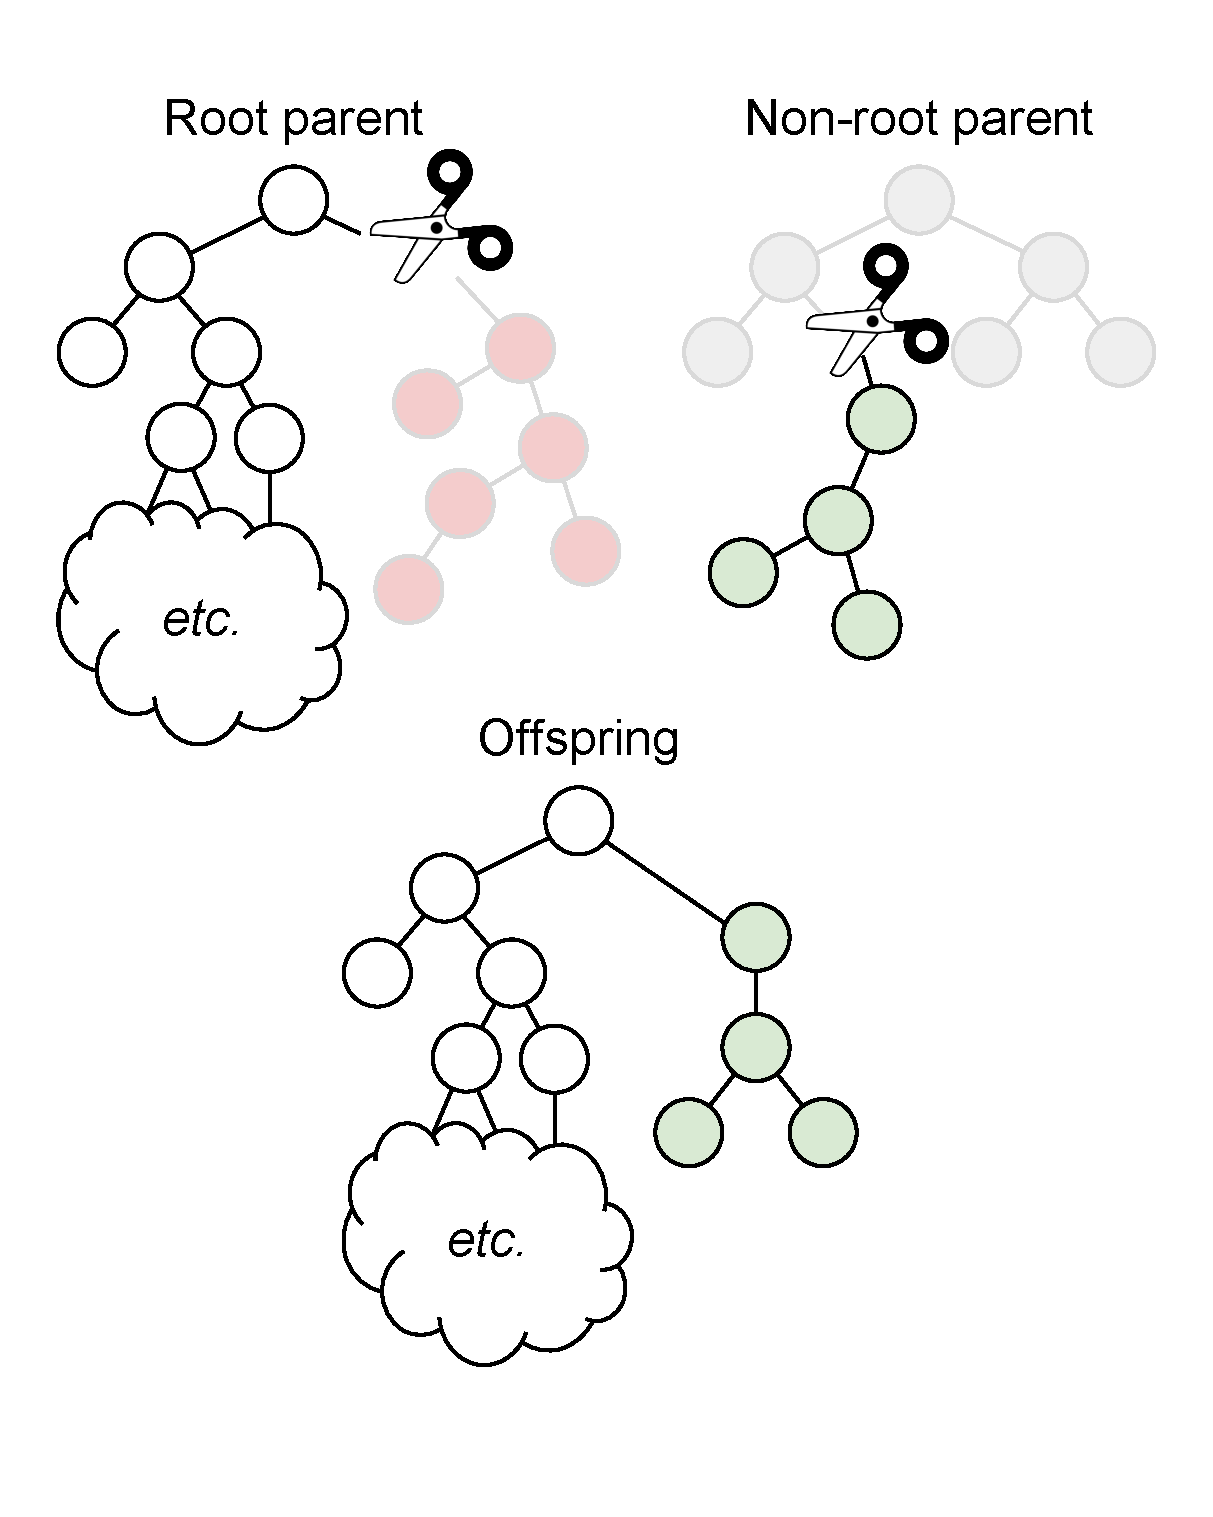
\includegraphics[width=0.35 \textwidth]{Plots/Root_parent_illustration_no_triangle.pdf}
	\caption{Sub-tree crossover, illustrating the asymmetric role of the \emph{root} and \emph{non-root} parents.}
	\label{fig:root_parent_illustration}
\end{figure}

An important impact of this asymmetry was recently noted in~\cite{McPheeDonatucciDramdahl:2014}, where it was observed
that the fitness of the offspring tended to improve when the root parent had better fitness than the non-root parent.
To explore this further, we implemented what we refer to as \emph{crossover bias}, which allowed us to
probabilistically force the GP system to assign the individual with the greater fitness to be the root parent. 
After reviewing some related work (Section~\ref{sec:relatedWork}),
we apply crossover bias (Section~\ref{sec:XObias}) to a variety of test problems
(Section~\ref{sec:Experiments}). The results (Section~\ref{sec:Results}) make it clear that crossover bias can have a
substantial impact on the performance of GP runs, but that the results are heavily parameter dependent and, to a lesser
degree problem dependent. In general, however, we find (Section~\ref{sec:Discussion}) that incorporating some crossover
bias is, at least in these problems, usually either advantageous or neutral.

\section{Related work}
\label{sec:relatedWork}

Several previous papers have deliberately created asymmetries between parents
(e.g.,~\cite{gohsexualselection,ryan1994pygmies}) as a mechanism to increase 
diversity and (in the case of~\cite{ryan1994pygmies}) combat bloat. 

There has also been a 
blossoming of work in the last few years based on the semantics of GP trees 
(e.g.,~\cite{McPhee:2008:SBB:1792694.1792707,moraglio2012geometric}). This includes a 
number of proposed mechanisms that encourage or force semantic differences (asymmetries) 
between parents and children~\cite{beadle2008semantically,uy2011semantically}. Some~\cite{uy2013roles} 
also \emph{limit} the differences between parents and offspring, in some sense reducing the impact 
of asymmetries between the parents, and smoothing out the fitness landscape as a result. These 
proposals typically focus on the semantic relationship between parents and children, however, and 
don't directly take into account any asymmetries between the parents.

\section{Crossover Bias} \label{sec:XObias}

To better understand parent asymmetries and the impact of bias in crossover, 
we implemented crossover bias with a parameter specifying the probability of forcing the more fit parent
to be the root parent when performing crossover, as detailed in Algorithm~\ref{alg:biasAlgorithm}. Every time a
crossover event was to be performed, we would use this probability to decide whether to force the more fit parent to be
the root parent. 
Note that when crossover bias isn't applied, there is still a 50\% chance that the root parent is the more fit
parent.

\begin{algorithm}[tb]
\begin{algorithmic}
\Require Two individuals are chosen as parents: RP (root parent) and NRP (non-root parent).
\If {\Call{random}{0, 1} $\leq \textrm{XO\_bias}$} \Comment{Do we force bias?}
    \If {\Call{fitness}{RP} \textrm{worse than} \Call{fitness}{NRP}}
        \State RP, NRP := NRP, RP \Comment{Swap so RP is more fit} 
    \EndIf
\EndIf
\end{algorithmic}
\caption{Crossover bias}
\label{alg:biasAlgorithm}
\end{algorithm}

In this paper we focus on five levels of crossover bias:
\begin{itemize}
\item 0.00 bias - no crossover bias is applied, i.e., just standard sub-tree crossover; 
	a 50\% probability of the more fit parent being the root parent;
\item 0.25 bias - system forced to use the more fit parent as the root parent in 25\% of cases; 
	a 62.5\% total probability of the more fit parent being the root parent;
\item 0.50 bias - system forced to use the more fit parent as the root parent in 50\% of cases; 
	a 75\% total probability of the more fit parent being the root parent;
\item 0.75 bias - system forced to use the more fit parent as the root parent in 75\% of cases; 
	a 87.5\% total probability of the more fit parent being the root parent; and
\item 1.00 bias - system forced to always use the more fit parent as the root parent, sometimes 
	referred to as ``with crossover bias''.
\end{itemize}

We also experimented with \emph{reverse bias}, where the weaker parent was always forced to be the root parent. In
general, the results for reverse bias showed no statistically significant difference from standard crossover (no bias),
so in the interest of simplification we've omitted reverse bias from the remainder of the paper.

\section{Experimental Setup} \label{sec:Experiments}

To better understand the impact of crossover bias on GP performance, we experimented with five problems: K Landscapes
with $K=6$~\cite{vanneschi2011k}, ORDER\-TREE~\cite{hoang2006ordertree}, U.S. Change, Sine
regression~\cite{poli08:fieldguide}, and Pagie-1 regression~\cite{pagie1997evolutionary}. Three of these (K Landscapes,
ORDERTREE, and Pagie-1 regression) are taken from recent benchmark suggestions~\cite{gp-benchmarks-2013}. The U.S. Change
problem \cite{zhan2014quantitative} has proven to be an interesting problem in evolutionary program
synthesis~\cite{Helmuth:GECCO15}, and sine regression is the example problem used in earlier work on the impact of
root and non-root parents~\cite{McPheeDonatucciDramdahl:2014}. 
All experiments were run using a copy of ECJ 21\footnote{\url{http://cs.gmu.edu/~eclab/projects/ecj/}} that we modified
to support crossover bias.

The one problem not precisely described elsewhere in the literature is the U.S. Change problem. Here the task is to
take as input an amount, and to return as output the minimum number of coins required to make that amount using (a
subset of) standard U.S. coins with amounts 25, 10, 5, and 1. So, for example, given 118 as input, the result should be
9 since 
\[
	\underline{4} \times 25 + \underline{1} \times 10 + \underline{1} \times 5 + \underline{3} \times 1 = 118,
\]
and this set of $4+1+1+3 = 9$ coins is the minimal set making a total of 118. Our function set for this problem was +,
-, $\times$, \%,\footnote{Protected integer division (quotient), returning 1 if the denominator is 0.} \emph{mod},\footnote{Also returns 1 if the denominator is 0.}
\emph{min}, and \emph{max}. The terminal set consisted of the input $x$, integer ephemeral random constants taken
uniformly from the range $[-50, 50]$, and the set of constants $\{ 0, 1, 4, 5, 9, 10, 24, 25 \}$. The test cases were
all inputs in the range $[0, 150)$.

% This is all taken from Tom Helmuth's version of the problem, and if the paper is accepted we should credit him in the
% camera ready copy.

All our experiments used the previously published settings, function sets, fitness functions, etc., with the 
exception of the parameters
listed in Table~\ref{tab:sharedParameters},\footnote{The function set for Pagie-1 specified
in~\cite{pagie1997evolutionary} is simply +, -, $\times$, and \% (protected division). The function set given
in~\cite{mcdermott2012genetic} and implemented in ECJ is ``koza2'', which also includes various trigonometric and
logarithmic functions. The performance of GP varies substantially between the two function sets; here we follow the
original Pagie-1 paper and use the simpler function set.} which are shared throughout these experiments. Our
evolutionary system is generational, with all new individuals being generated via subtree crossover (i.e., no mutation
or reproduction) unless there is a non-zero elitism percentage. Our primary goal was to better understand the impact of
crossover bias, so we performed runs with a variety of crossover bias probabilities. In addition, we wanted to see how
crossover bias might interact with some other commonly manipulated parameters as listed in
Table~\ref{tab:sharedParameters}. Unless otherwise noted, all plots, etc., in what follows will include results from
all possible combinations of values in Table~\ref{tab:sharedParameters}. Each box plot in
Figure~\ref{fig:KLandscapes6_results}, for example, includes the results of 100 runs for each of the combinations of
all four tournament sizes, both elitism proportions, and both population sizes.

\begin{table}[tb]
\begin{center}
\begin{tabular}{ll}
\textbf{Parameter} & \textbf{Values} \\
% \hline
Crossover bias & 0, 0.25, 0.5, 0.75, and 1 \\
Tournament size & 2, 3, 5, and 7 \\
Elitism \% & 0 and 1\% \\
Population size & 1,024 and 10,240 \\
\# of generations & 100 \\
\# of runs per treatment & 100
\end{tabular}
\end{center}
\vspace{-0.5cm}
\caption{Shared parameters}
\label{tab:sharedParameters}
\end{table}

In our experimentation we observed that
there were quite substantial interactions between crossover bias and some of
the other parameter settings. In particular, we found that there are parameter values where crossover bias appears to
have a substantial and significant impact, and other parameter settings where crossover bias has almost no effect on
the results. Based on these observed patterns, we found it useful to identify two specific subsets of the parameter
settings listed in Table~\ref{tab:sharedParameters}: ``\emph{bias-effective settings}'' and ``\emph{non-bias-effective
settings}''. The bias-effective settings are binary tournaments, no elitism, and population size of 10,240; the
non-bias-effective settings, conversely, are tournament size 7, non-zero elitism percentage, and population size 1,024.
These terms will be used in the remainder of the paper, which will also include some discussion of why crossover bias
might interact with these parameters in this way.

To illustrate the impact of these parameter settings, 
Figure~\ref{fig:sineFitnessVsGenFacets} shows the fitness (absolute error) over time for the sine regression problem
(see Section~\ref{sec:sineRegression} for more on the sine regression results). 
The bias-effective settings (left-hand panel) show a clear difference in the performance as a function of 
crossover bias, where the non-bias-effective settings (right hand panel) show almost no difference as a function of
the crossover bias probability.

\begin{figure}
	\centering
	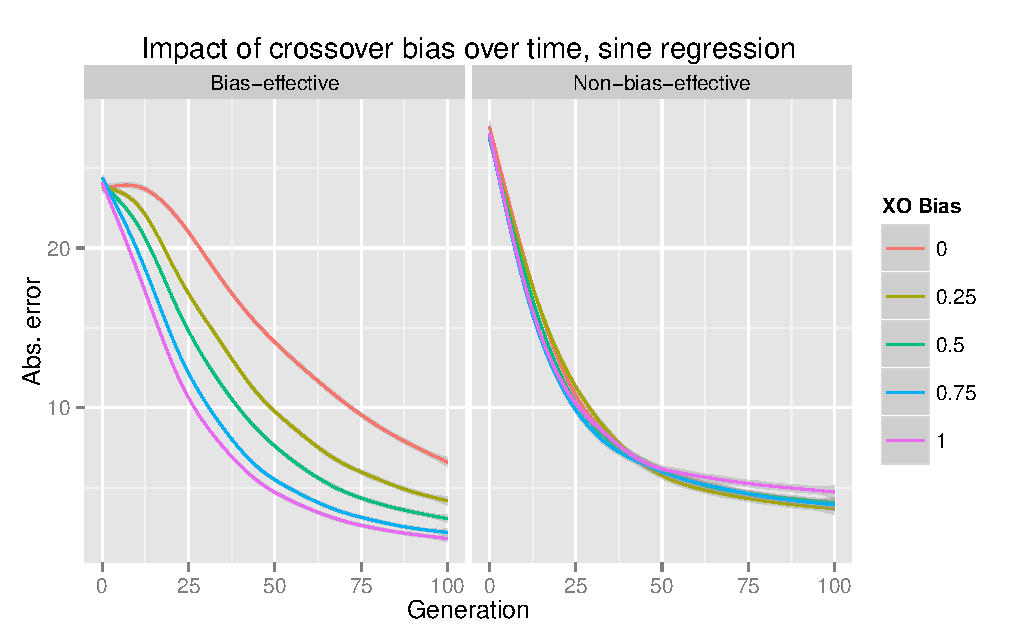
\includegraphics[width=0.45 \textwidth]{Plots/Sine_fitness_vs_gen_facets.pdf}
	\caption{Impact of crossover bias over time on the sine symbolic regression problem with
		\emph{bias-effective} and \emph{non-bias-effective} parameter sets. In the left-hand panel (bias-effective settings), the curves stack in order (top to bottom) from crossover bias 0 to crossover bias 1.}
	\label{fig:sineFitnessVsGenFacets}
\end{figure}

\section{Results} \label{sec:Results}

All tests of differences in fitness or hits in this section are performed using pairwise Wilcoxon tests with Holm
corrections. Tests of differences in the number of successes are performed using pairwise tests of proportions
(chi-squared) with Holm corrections. All statistics calculations were performed with R~\cite{R} and all plots were
generated using the ggplot2 package~\cite{ggplot2Book}. Statistical significance will require $p \leq 0.05$.

\subsection{Structural Problems}

Most GP problems evaluate the evolved trees on a set of inputs, looking for some desired behavior or semantics.
Structural problems (also referred to as constructed problems), however, have fitness functions that are entirely 
based on the overall structure of the evolved trees (e.g., size, shape, distribution of particular leaves) without 
any sort of ``evaluation" being involved.

\subsubsection{K Landscapes Problem}

Fitnesses for the K Landscape problem are between 0 and 1, with a fitness of 1 being a perfect solution.
Figure~\ref{fig:KLandscapes6_results} shows the impact of crossover bias on this problem across all the combinations of
parameter values in Table~\ref{tab:sharedParameters}. Increasing the amount of crossover bias consistently improves the
fitness of the results. All the differences are statistically significant ($p < 0.012$) except for the difference
between bias probability 0.75 and 1.00.

%> pairwise.wilcox.test(klandscapes6$Fitness, klandscapes6$Bias.probability)
%
%	Pairwise comparisons using Wilcoxon rank sum test 
%
%data:  klandscapes6$Fitness and klandscapes6$Bias.probability 
%
%     -1      0       0.25    0.5     0.75   
%0    0.99997 -       -       -       -      
%0.25 1.8e-06 1.8e-06 -       -       -      
%0.5  1.7e-12 2.3e-12 0.01136 -       -      
%0.75 < 2e-16 < 2e-16 6.0e-10 0.00032 -      
%1    < 2e-16 < 2e-16 3.7e-15 2.2e-07 0.15773
%
%P value adjustment method: holm 

\begin{figure}[t]
\centering
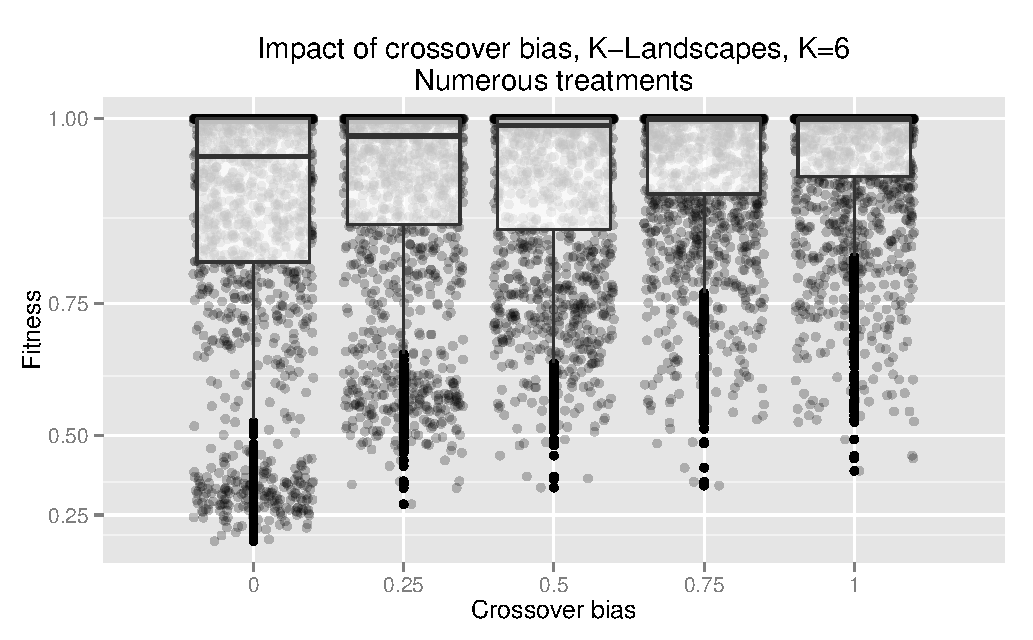
\includegraphics[width=0.45 \textwidth]{Plots/KLandscapes6_XO_bias_impact_transformed_boxplot_alpha075.pdf}
\caption{Impact of crossover bias on fitness for the K Landscapes problem, over all the combinations of 
	parameters in Table~\ref{tab:sharedParameters}.}
\label{fig:KLandscapes6_results}
\end{figure}

Compare this to the results shown in Figure~\ref{fig:KLandscapes6_XO_bias_impact_facets}, which plots the same data
separated out by tournament size. It is clear that for binary tournaments, increasing the crossover bias probability
continues to improve the fitness -- all the differences are strongly statistically significant ($p<6\times 10^{-08}$).
This continues to be true for tournament size 3; all the differences are statistically significant except for those
between bias 0.50 and 0.75, which was very close ($p=0.056$). None of the differences for tournament size 5 are
significant. For tournament size 7, however, it looks like the reverse is true, where increasing crossover bias actually
hurts fitness. Almost none of the differences for tournament size 7 are statistically significant with the only
exception being the difference between 0.25 and 1.00 ($p=0.021$).

\begin{figure}[t]
\centering
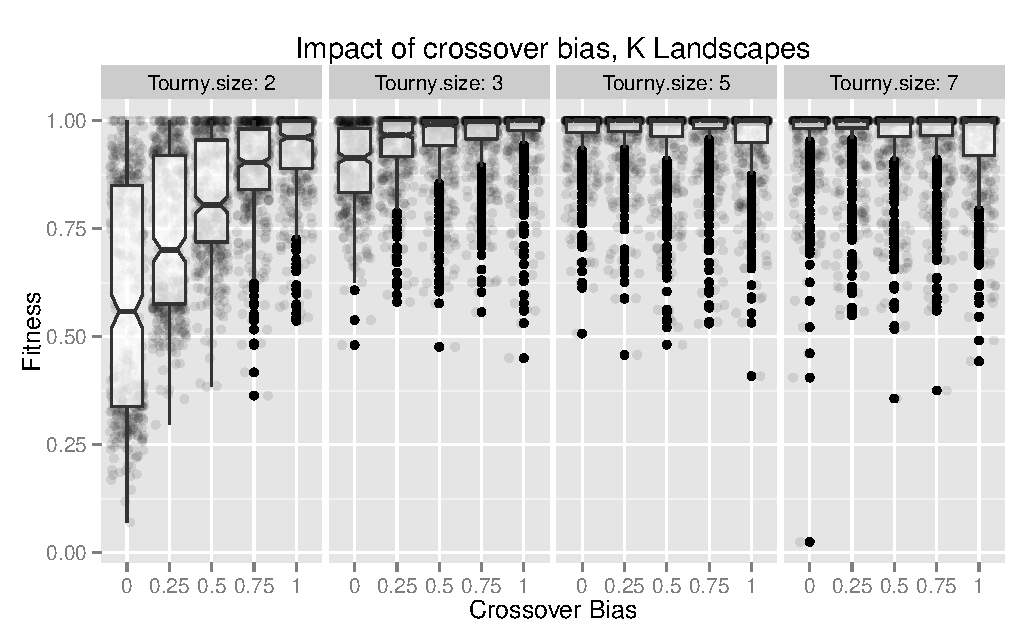
\includegraphics[width=0.45 \textwidth]{Plots/KLandscapes6_XO_bias_impact_facets.pdf}
\caption{Impact of crossover bias on fitness for the K Landscapes problem, for various tournament sizes.}
\label{fig:KLandscapes6_XO_bias_impact_facets}
\end{figure}

Figure~\ref{fig:KLandscapes6_strong_results} filters out only the data gathered using the bias-effective treatment,
as defined in Section~\ref{sec:Experiments}. It is clear that the impact of crossover bias is much stronger in this case
than in the more general case shown in Figure~\ref{fig:KLandscapes6_results}. Here all the differences are strongly
statistically significant ($p < 10^{-11}$). In addition to improvements in fitness, increasing the crossover bias also
increases the number of ``perfect'' solutions discovered when using the bias effective settings. 
Out of 100 runs with a crossover bias setting of 1.00, 15 of
these runs resulted in the discovery of a ``perfect'' solution. By comparison, only 1 or 2 runs out of 100 resulted in
``perfect'' solutions for each of the other crossover bias probabilities. 
These differences in the number of perfect solutions are statistically significant
($p \leq 0.03$).

\begin{figure}[t]
\centering
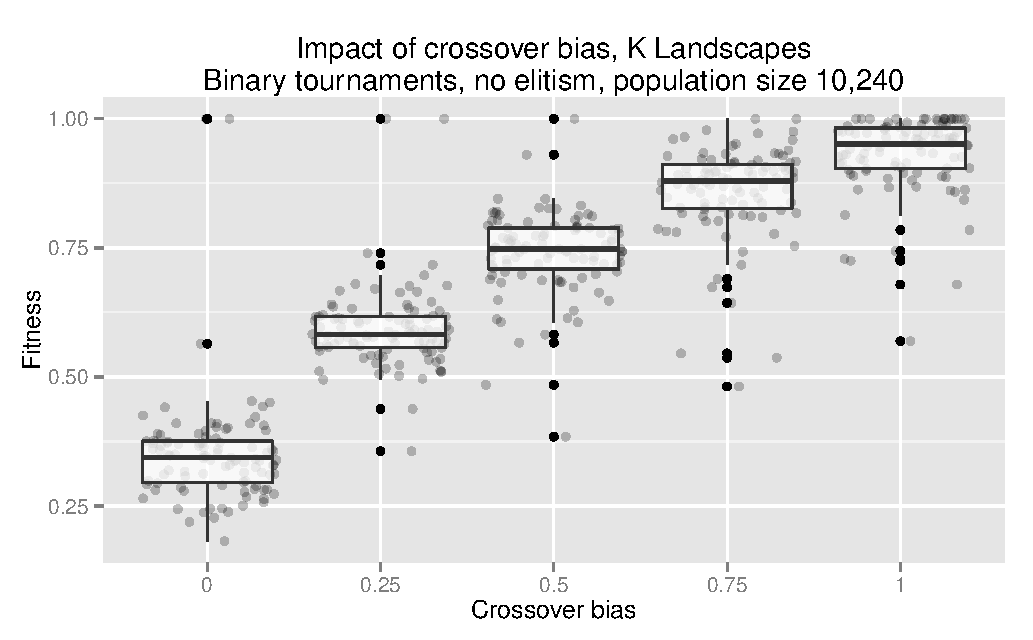
\includegraphics[width=0.45 \textwidth]{Plots/KLandscapes6_XO_bias_strong_impact_alpha_075.pdf}
\caption{Impact of crossover bias on fitness for the K Landscapes problem, restricted to bias-effective parameter settings.}
\label{fig:KLandscapes6_strong_results}
\end{figure}

%> pairwise.wilcox.test(strong$Fitness, strong$Bias.probability)
%
%	Pairwise comparisons using Wilcoxon rank sum test 
%
%data:  strong$Fitness and strong$Bias.probability 
%
%     -1      0       0.25    0.5     0.75   
%0    0.18    -       -       -       -      
%0.25 < 2e-16 < 2e-16 -       -       -      
%0.5  < 2e-16 < 2e-16 < 2e-16 -       -      
%0.75 < 2e-16 < 2e-16 < 2e-16 < 2e-16 -      
%1    < 2e-16 < 2e-16 < 2e-16 < 2e-16 2.3e-12
%
%P value adjustment method: holm 

%> countSuccesses(strong)
%[1]  1  2  2  1  2 15
%> pairwise.prop.test(countSuccesses(strong), rep(100, 6))
%
%	Pairwise comparisons using Pairwise comparison of proportions 
%
%data:  countSuccesses(strong) out of rep(100, 6) 
%
%  1     2     3     4     5    
%2 1.000 -     -     -     -    
%3 1.000 1.000 -     -     -    
%4 1.000 1.000 1.000 -     -    
%5 1.000 1.000 1.000 1.000 -    
%6 0.011 0.030 0.030 0.011 0.030
%
%P value adjustment method: holm 

\subsubsection{ORDERTREE Problem}

It should be noted that, for the ORDERTREE problem we used the full set of parameters outlined in
Section~\ref{sec:Experiments}, with one exception: the population size for the ORDERTREE runs was limited to 1,024.
This was a consequence of the large trees generated for this problem, resulting in out of memory errors for the larger
population size of 10,240. 

ORDERTREE has a difficulty tuning parameter $n$; we used $n=10$, which meant that the fitnesses ranged from 
0 to 1,022 with larger values being better. The details for the ORDERTREE fitness 
computation are described in~\citep{hoang2006ordertree}.

Figure~\ref{fig:Ordertree_results_all_tournaments_Jan15} shows the impact of crossover bias across all parameter 
combinations. 
For binary tournaments, adding crossover bias leads to improved performance when compared to no crossover bias,
but we observed a drop in fitness from bias 0.75 to
bias 1.00, where the fitness for 1.00 is actually slightly below that for 0.50 as well. All the binary tournament 
differences are
statistically significant ($p < 0.03$), with the exception of the difference between bias 0.25 and bias 1.00, so bias
0.75 is the clear winner in this scenario. This drop in fitness for bias 1.00 is consistent across the other three
tournament sizes as well. However, it is also apparent from the figure that in general the impact of crossover bias
lessens with the larger tournament sizes, both in the increase in fitness up to bias 0.75, and the drop from there to
bias 1.00.

\begin{figure}
\centering
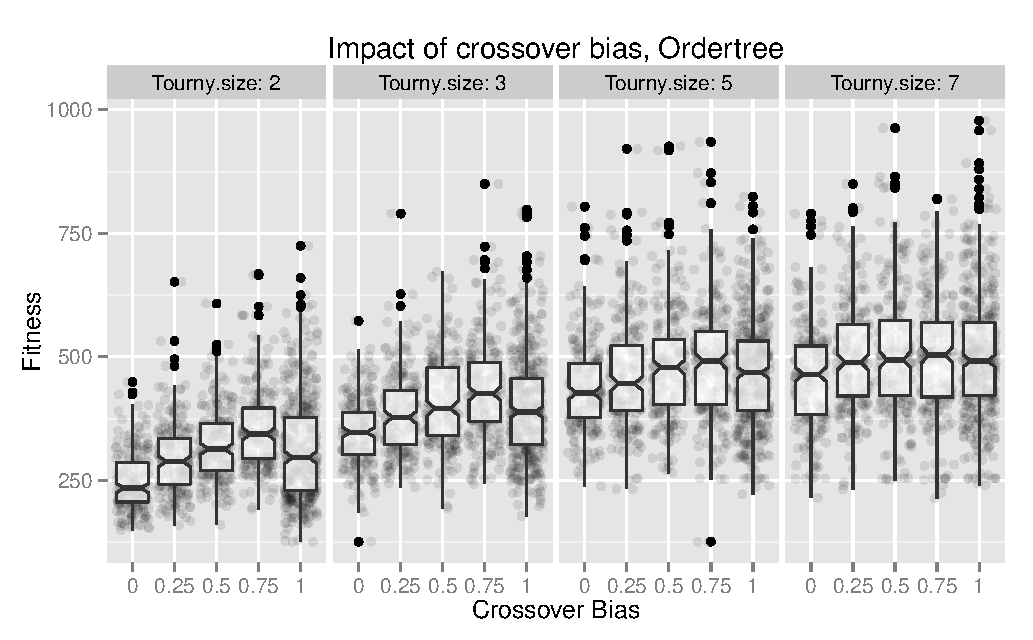
\includegraphics[width=0.45 \textwidth]{Plots/Ordertree_results_all_tournaments_Jan15.pdf}
\caption{Impact of crossover bias on fitness for \mbox{ORDERTREE} problem for multiple tournament sizes.}
\label{fig:Ordertree_results_all_tournaments_Jan15}
\end{figure}

%> pairwise.wilcox.test(subset(klandscapes6, Tourny.size==7)$Fitness, subset(klandscapes6,
%Tourny.size==7)$Bias.probability)
%
%	Pairwise comparisons using Wilcoxon rank sum test 
%
%data:  subset(klandscapes6, Tourny.size == 7)$Fitness and subset(klandscapes6, Tourny.size == 7)$Bias.probability 
%
%     0     0.25  0.5   0.75 
%0.25 1.000 -     -     -    
%0.5  1.000 1.000 -     -    
%0.75 1.000 0.556 1.000 -    
%1    0.075 0.021 0.556 1.000
%
%P value adjustment method: holm 

\subsection{U.S. Change Problem} \label{sec:USChange}

In contrast to the structural problems discussed in the previous section, which used fitness as the measure of success
of a run, for the U.S. Change problem we measured success in ``hits'' (the number of test cases that are correctly
solved). There are 150 test cases in our implementation, so an optimal program will have a score of 150 hits.

Figure~\ref{fig:USChange_Hits} shows the impact of crossover bias on the number of hits for the U.S. Change problem
across the full collection of parameter settings. This suggests that in general there is little consistent impact of
crossover bias; while most of the differences in this plot are not statistically significant, two are: the differences
between crossover bias 0.00 and crossover bias 0.50 and 0.75 are both statistically significant ($p \leq 0.015$), even
if numerically small.

\begin{figure}[tb]
\centering
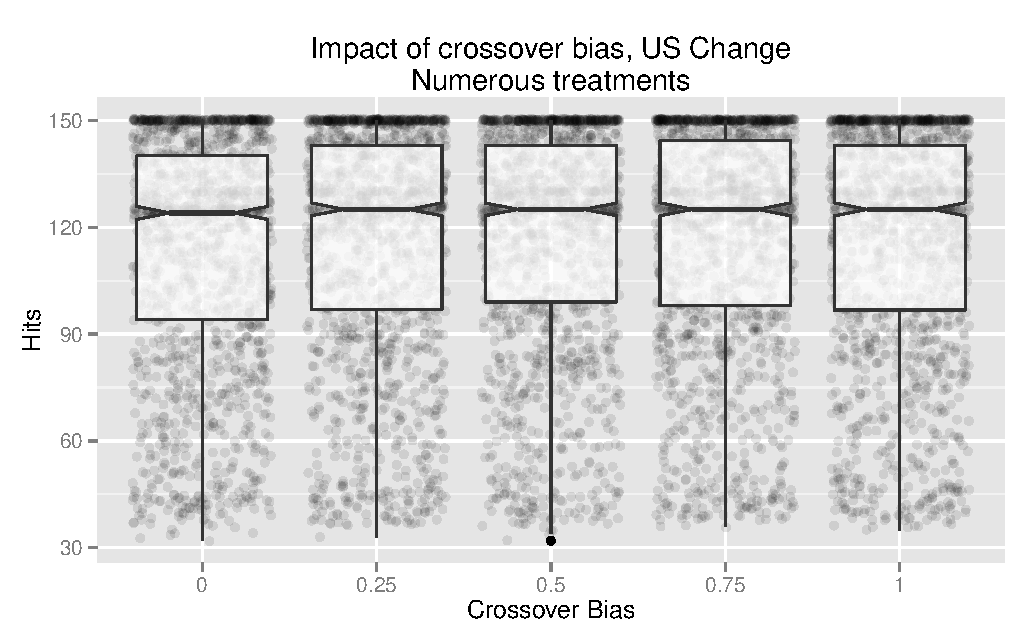
\includegraphics[width=0.45 \textwidth]{Plots/US_change_hits.pdf}
\caption{Impact of crossover bias on the number of hits for the U.S. Change problem for all the combinations 
	of parameters in Table~\ref{tab:sharedParameters}.}
\label{fig:USChange_Hits}
\end{figure}

%> pairwise.wilcox.test(us_change$Hits, us_change$Bias, conf.int=TRUE)
%
%	Pairwise comparisons using Wilcoxon rank sum test 
%
%data:  us_change$Hits and us_change$Bias 
%
%     0     0.25  0.5   0.75 
%0.25 0.117 -     -     -    
%0.5  0.011 1.000 -     -    
%0.75 0.015 1.000 1.000 -    
%1    0.083 1.000 1.000 1.000
%
%P value adjustment method: holm 

However, if we limit our attention to the bias-effective parameter settings defined in Section~\ref{sec:Experiments}, then we
find that crossover bias has a substantial and statistically significant impact, as is seen in
Figure~\ref{fig:USChange_Hits_strong}. Here the bulk of these pairwise differences are statistically significant
($p<0.0002$). The major exception is the difference between crossover bias 0.75 and 1.00 ($p=0.43$). Two other
adjacent pairs have $p$-values slightly above 0.05: crossover bias 0.25 \emph{vs.}\ 0.50 ($p=0.0504$), and 0.50
\emph{vs.}\ 0.75 ($p=0.0802$).

\begin{figure}[tb]
\centering
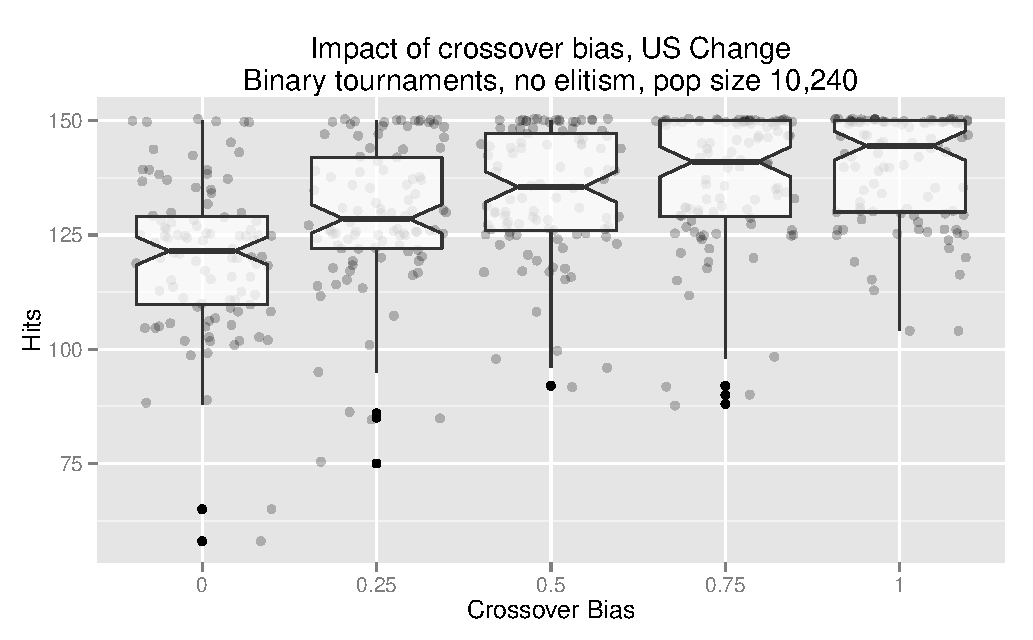
\includegraphics[width=0.45 \textwidth]{Plots/US_change_hits_strong.pdf}
\caption{Impact of crossover bias on the number of hits for the U.S. Change problem, limited to bias-effective
parameters.}
\label{fig:USChange_Hits_strong}
\end{figure}

%> pairwise.wilcox.test(us_change_strong$Hits, us_change_strong$Bias)
%
%	Pairwise comparisons using Wilcoxon rank sum test 
%
%data:  us_change_strong$Hits and us_change_strong$Bias 
%
%     0       0.25    0.5     0.75   
%0.25 0.00013 -       -       -      
%0.5  3.4e-09 0.05036 -       -      
%0.75 1.1e-12 0.00016 0.08019 -      
%1    3.2e-15 5.1e-06 0.01652 0.43078
%
%P value adjustment method: holm 

If complete success was considered vital (which might be the case if we were evolving software for use in a production
system), then it would make sense to see if crossover bias has a significant impact on the success rate.
Figure~\ref{fig:USChange_Successes_strong} shows the number of successes for the various crossover bias values when
using the bias-effective parameter settings. None of the adjacent differences (for example, crossover bias 0.50
\emph{vs.}\ 0.75) are statistically significant, while most of the non-adjacent differences (for example, crossover bias
0.25 \emph{vs.}\ 0.75) are statistically significant, with the exceptions being crossover bias 0.00 \emph{vs.}\ 0.50, and
bias 0.50 \emph{vs.}\ 1.00 ($p=0.094$ in both cases).

\begin{figure}
\centering
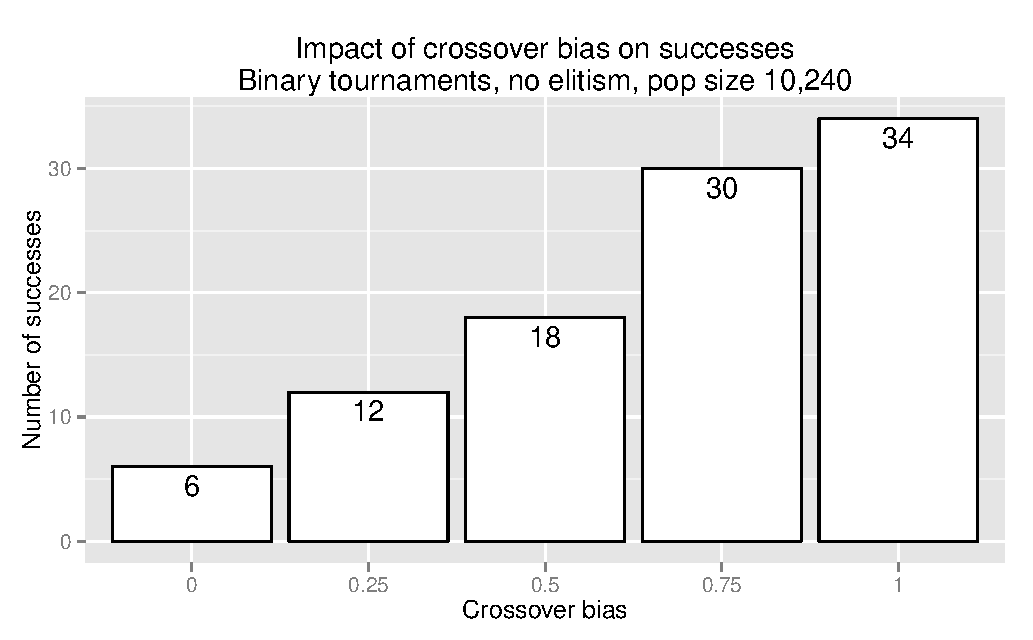
\includegraphics[width=0.45 \textwidth]{Plots/US_change_successes_strong.pdf}
\caption{Impact of crossover bias on the number of successful runs for the U.S. Change problem when using
bias-effective parameters.}
\label{fig:USChange_Successes_strong}
\end{figure}

%> pairwise.prop.test(c(6, 12, 18, 30, 34), rep(100, 5))
%
%	Pairwise comparisons using Pairwise comparison of proportions 
%
%data:  c(6, 12, 18, 30, 34) out of rep(100, 5) 
%
%  1       2       3       4      
%2 0.65003 -       -       -      
%3 0.09361 0.65003 -       -      
%4 0.00021 0.02215 0.27429 -      
%5 1.8e-05 0.00334 0.09361 0.65003
%
%P value adjustment method: holm 

%\begin{figure}
%\centering
%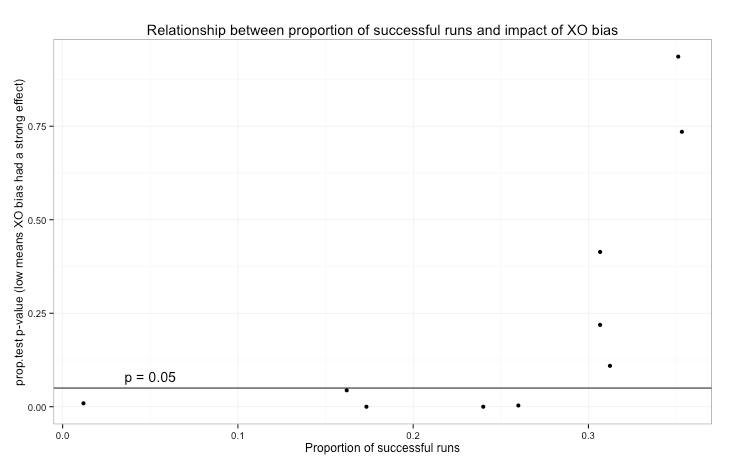
\includegraphics[width=0.45 \textwidth]{Plots/US_change_Bias_impact_vs_success.png}
%\caption{Relationship between proportion of successful runs and the impact of crossover bias.}
%\label{fig:USChangeBiasImpactVsSuccess}
%\end{figure}

\subsection{Regression Problems}

Regression problems attempt to evolve a function that is able to match a given set of input-output pairs. 
Success is here measured in hits, where a ``hit'' is awarded when the output of the evolved function is within 0.01
of the target value.

\subsubsection{Pagie-1 Problem}

Figure~\ref{fig:Pagie1Hits_Bias_Tournys_FunctionSet} shows the impact of crossover bias on the number of hits for the
Pagie-1 regression problem, separated out by tournament size. 
Figure~\ref{fig:Pagie1StrongHits_Bias_Tournys_FunctionSet} is limited  to population size 10,240
and no elitism.

\begin{figure}[tb]
\centering
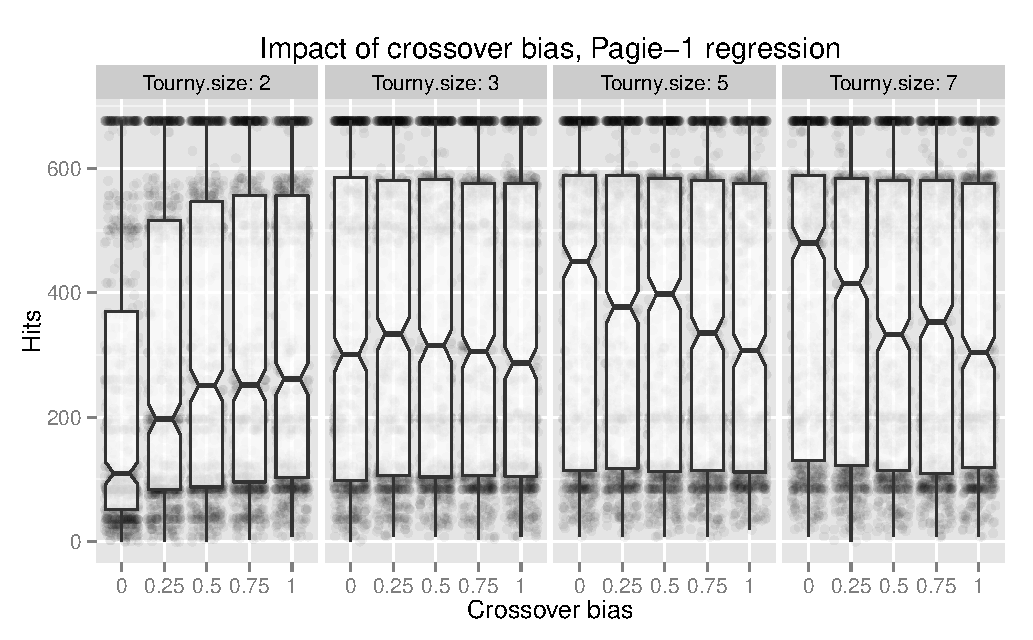
\includegraphics[width=0.45 \textwidth]{Plots/Pagie_1_Hits_vs_Bias_Tournys.pdf}
\caption{Impact of crossover bias on the number of hits for the Pagie-1 symbolic regression problem, 
	broken out across the four different tournament sizes. The maximum number of possible hits is 676.}
\label{fig:Pagie1Hits_Bias_Tournys_FunctionSet}
\end{figure}

\begin{figure}[tb]
\centering
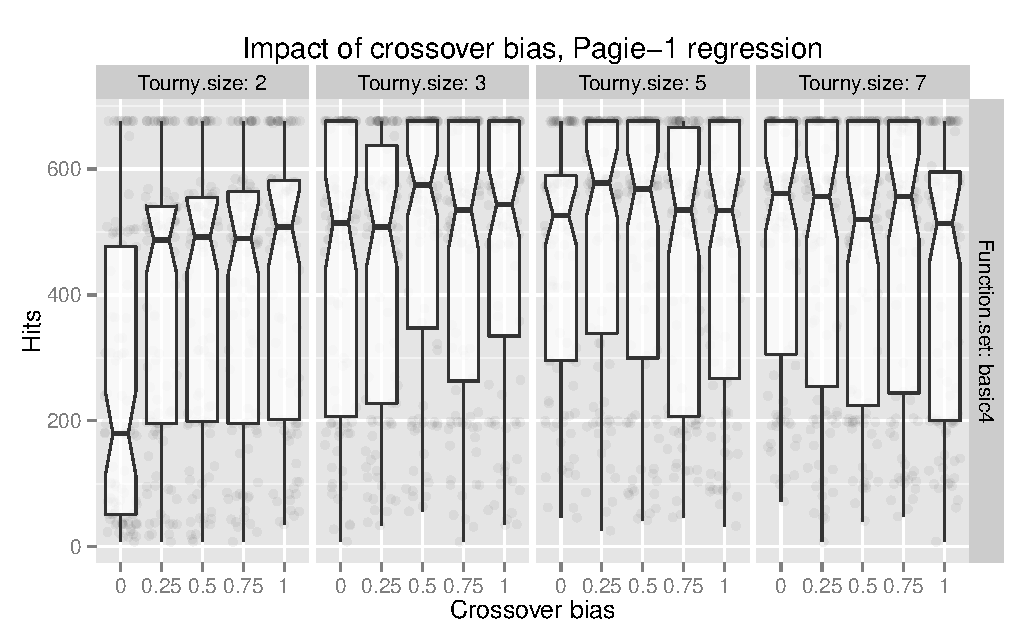
\includegraphics[width=0.45\textwidth]
{Plots/Pagie_1_strong_No_Tarpeian_Hits_vs_Bias_Tournys_FunctionSet.pdf}
\caption{Impact of crossover bias on the number of hits for the Pagie-1 symbolic regression problem, 
	broken out by tournament size, limited to bias-effective elitism (0) and population size (10,240).}
\label{fig:Pagie1StrongHits_Bias_Tournys_FunctionSet}
\end{figure}

Focusing on the binary tournament data in Figure~\ref{fig:Pagie1StrongHits_Bias_Tournys_FunctionSet}, the differences
between crossover bias 0.00 (standard subtree crossover) and all the other positive crossover bias values are
statistically significant ($p<0.0002$). 
None of the differences among 0.25, 0.50, 0.75, and 1.00 are statistically significant, however, and
none of the differences for tournament sizes 3, 5, or 7 are statistically significant. This indicates that for binary
tournaments, including crossover bias substantially and significantly improves the hit rate, although all bias rates
above 0.25 are very similar. For larger tournament sizes, however, it appears that adding crossover bias doesn't have a significant effect and in some cases (e.g., tournament sizes 5 and 7 in Figure~\ref{fig:Pagie1Hits_Bias_Tournys_FunctionSet}) may hurt performance.

%> pairwise.wilcox.test(subset(pagie1_strong_no_Tarpeian, Tourny.size==2)$Hits, 
%+                      subset(pagie1_strong_no_Tarpeian, Tourny.size==2)$Bias)
%
%Pairwise comparisons using Wilcoxon rank sum test 
%
%data:  subset(pagie1_strong_no_Tarpeian, Tourny.size == 2)$Hits and subset(pagie1_strong_no_Tarpeian, Tourny.size == 2)$Bias 
%
%0       0.25   0.5    0.75  
%0.25 0.0002  -      -      -     
%0.5  2.6e-05 1.0000 -      -     
%0.75 5.1e-06 1.0000 1.0000 -     
%1    9.9e-08 0.5505 0.9863 1.0000
%
%P value adjustment method: holm 

\pagebreak

\subsubsection{Sine Problem}
\label{sec:sineRegression}

For the sine regression problem, we limited our runs to bias-effective and non-bias-effective settings as defined in Section~\ref{sec:Experiments}.

Figure~\ref{fig:sineBiasResultsStrong} shows the results for the number of hits 
for the sine regression problem using bias-effective
settings. All these differences are statistically significant ($p < 10^{-5}$) except for the difference between the
bias of 0.75 and 1.00. In Figure~\ref{fig:sineFitnessVsGenFacets}, the left panel illustrates the impact of crossover
bias over time when using the bias-effective settings, demonstrating that the effects appear early in the run. Here,
the fitnesses are consistently different throughout the time of the runs, with higher crossover bias settings arriving
at fitter individuals earlier in the runs, although the differences are shrinking towards the end as many runs find
fairly fit individuals.

\begin{figure}[t]
\centering
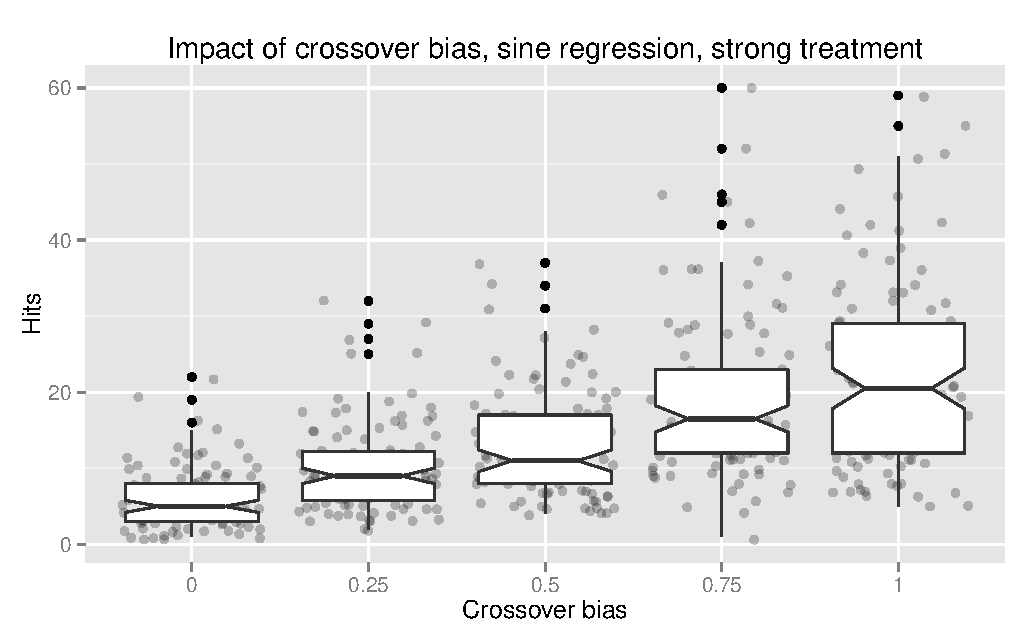
\includegraphics[width=0.45 \textwidth]{Plots/Sine_XO_impact_strong_boxplot.pdf}
\caption{Impact of crossover bias on the sine symbolic regression problem with bias-effective settings.}
\label{fig:sineBiasResultsStrong}
\end{figure}

%> pairwise.wilcox.test(sine_strong_final$Hits, sine_strong_final$Bias)
%
%	Pairwise comparisons using Wilcoxon rank sum test 
%
%data:  sine_strong_final$Hits and sine_strong_final$Bias 
%
%     0       0.25    0.5     0.75  
%0.25 1.9e-07 -       -       -     
%0.5  4.0e-15 0.0017  -       -     
%0.75 < 2e-16 1.2e-12 8.9e-06 -     
%1    < 2e-16 1.3e-13 2.9e-07 0.1938
%
%P value adjustment method: holm 

%> pairwise.wilcox.test(sine_strong_final$Standardized.fitness, sine_strong_final$Bias)
%
%	Pairwise comparisons using Wilcoxon rank sum test 
%
%data:  sine_strong_final$Standardized.fitness and sine_strong_final$Bias 
%
%     0       0.25    0.5     0.75 
%0.25 3.6e-10 -       -       -    
%0.5  < 2e-16 2.7e-05 -       -    
%0.75 < 2e-16 5.0e-14 1.1e-05 -    
%1    < 2e-16 < 2e-16 2.9e-09 0.072
%
%P value adjustment method: holm 

Figure~\ref{fig:sineBiasResultsWeak} shows the results for the sine regression problem using the non-bias-effective
parameter settings; none of these differences are
statistically significant. In Figure~\ref{fig:sineFitnessVsGenFacets}, the right panel illustrates the impact of
crossover bias over time when using the non-bias-effective settings, demonstrating that with these settings the runs
tend to be highly similar throughout the duration of the runs, regardless of crossover bias setting. 

% I don't think that the following is actually supported by this plot, although it *might* be
% supported by the plot with the 10K pop size. - Nic
%However, in what little variation does exist between the runs, the
%figure shows that while higher crossover bias settings tend to produce slightly fitter individuals toward the beginning
%of the runs, this trend is reversed by the end of the runs.

\begin{figure}[t]
\centering
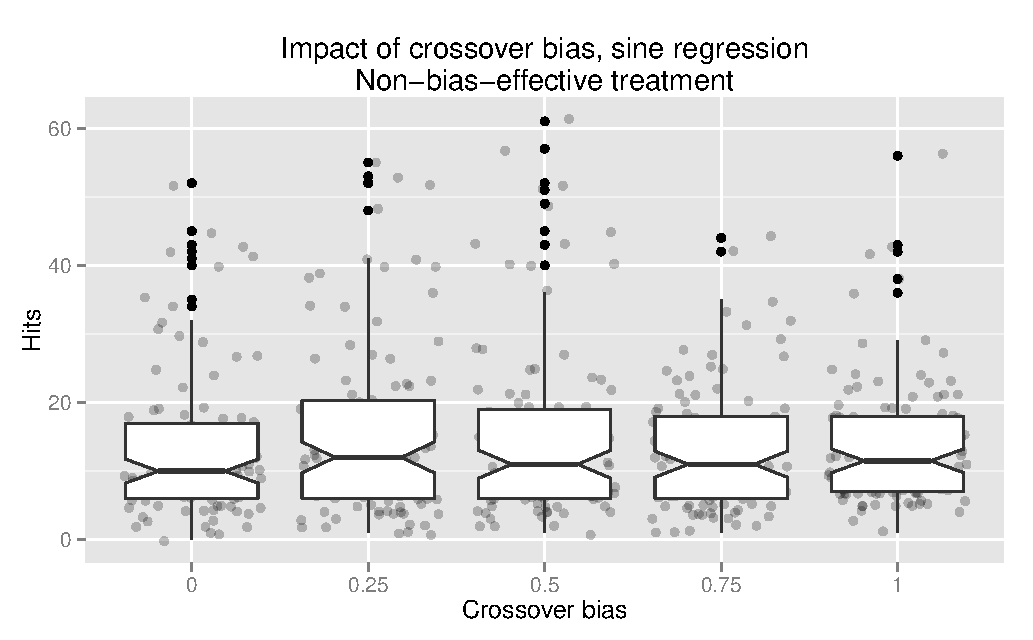
\includegraphics[width=0.45 \textwidth]{Plots/Sine_XO_impact_weak_e01_boxplot.pdf}
\caption{Impact of crossover bias on the sine symbolic regression problem with non-bias-effective settings.}
\label{fig:sineBiasResultsWeak}
\end{figure}

\pagebreak

\section{Discussion} \label{sec:Discussion}

In general our results indicate that adding crossover bias improves performance, either generally
(Figure~\ref{fig:KLandscapes6_results}) or when combined with certain other parameter choices (e.g.,
Figure~\ref{fig:Pagie1Hits_Bias_Tournys_FunctionSet}). In some cases the improvements induced by crossover bias are
quite substantial (e.g., Figures~\ref{fig:KLandscapes6_strong_results},~\ref{fig:USChange_Successes_strong},
and~\ref{fig:sineBiasResultsStrong}), while in other situations the improvements were quite small in magnitude even
when statistically significant (Figure~\ref{fig:KLandscapes6_results}). Not surprisingly, however, crossover bias is
not universally helpful, and there are settings where some crossover bias improves performance more than when always
applying crossover bias (Figure~\ref{fig:Ordertree_results_all_tournaments_Jan15}), and other settings where all tested
crossover bias amounts were detrimental (tournament sizes 5 and 7 in
Figure~\ref{fig:Pagie1Hits_Bias_Tournys_FunctionSet}).

One general trend seems to be that crossover bias is more effective when using the \emph{bias-effective} parameter
settings, namely smaller tournaments (size 2 instead of 7), larger populations (10,240 instead of 1,024), and no
elitism. One possible explanation for this pattern is that when using the \emph{non-bias-effective} settings, 
the difference in fitness between the two parents is likely to be
closer than when using bias-effective settings; this reduction in the difference between the fitness of the 
parents is thus likely to minimize the impact of crossover bias.

%Larger tournaments, for example, help ensure that both parents are from the more highly fit part of the population,
%especially when using smaller population sizes. 

To test this hypothesis, we looked at the impact of tournament size on the relative difference in parent fitness for
the K Landscapes problem and the sine regression problem. For each crossover event, we compute the relative difference
in parent fitness as
\[
	|f_A - f_B| / (f_A + f_B)
\]
where $f_A$ and $f_B$ are the fitnesses of the two chosen parents $A$ and $B$. This has a minimum value of 0 when the two
fitnesses are the same, and a maximum value approaching 1 for the case where one of the values is nearly 0.

Figure~\ref{fig:parentDiffsKLandscapes} shows the distribution of the relative differences in parent fitness for the K
Landscapes problem both with (right-hand panel) and without (left-hand panel) crossover bias. 
For tournament size 7, the difference in fitness drops
significantly as the run progresses; this, combined with the substantial improvements in fitness, suggests that 
both of the parents are highly fit. When using binary
tournaments, the relative differences in parent fitness remains fairly stable and higher than for tournament size 7, 
which would suggest that
crossover bias would continue to be effective throughout the run when using binary tournaments. We see similar results
in the sine regression problem, as illustrated in Figure~\ref{fig:parentDiffsSine}.

\begin{figure}[tb]
\centering
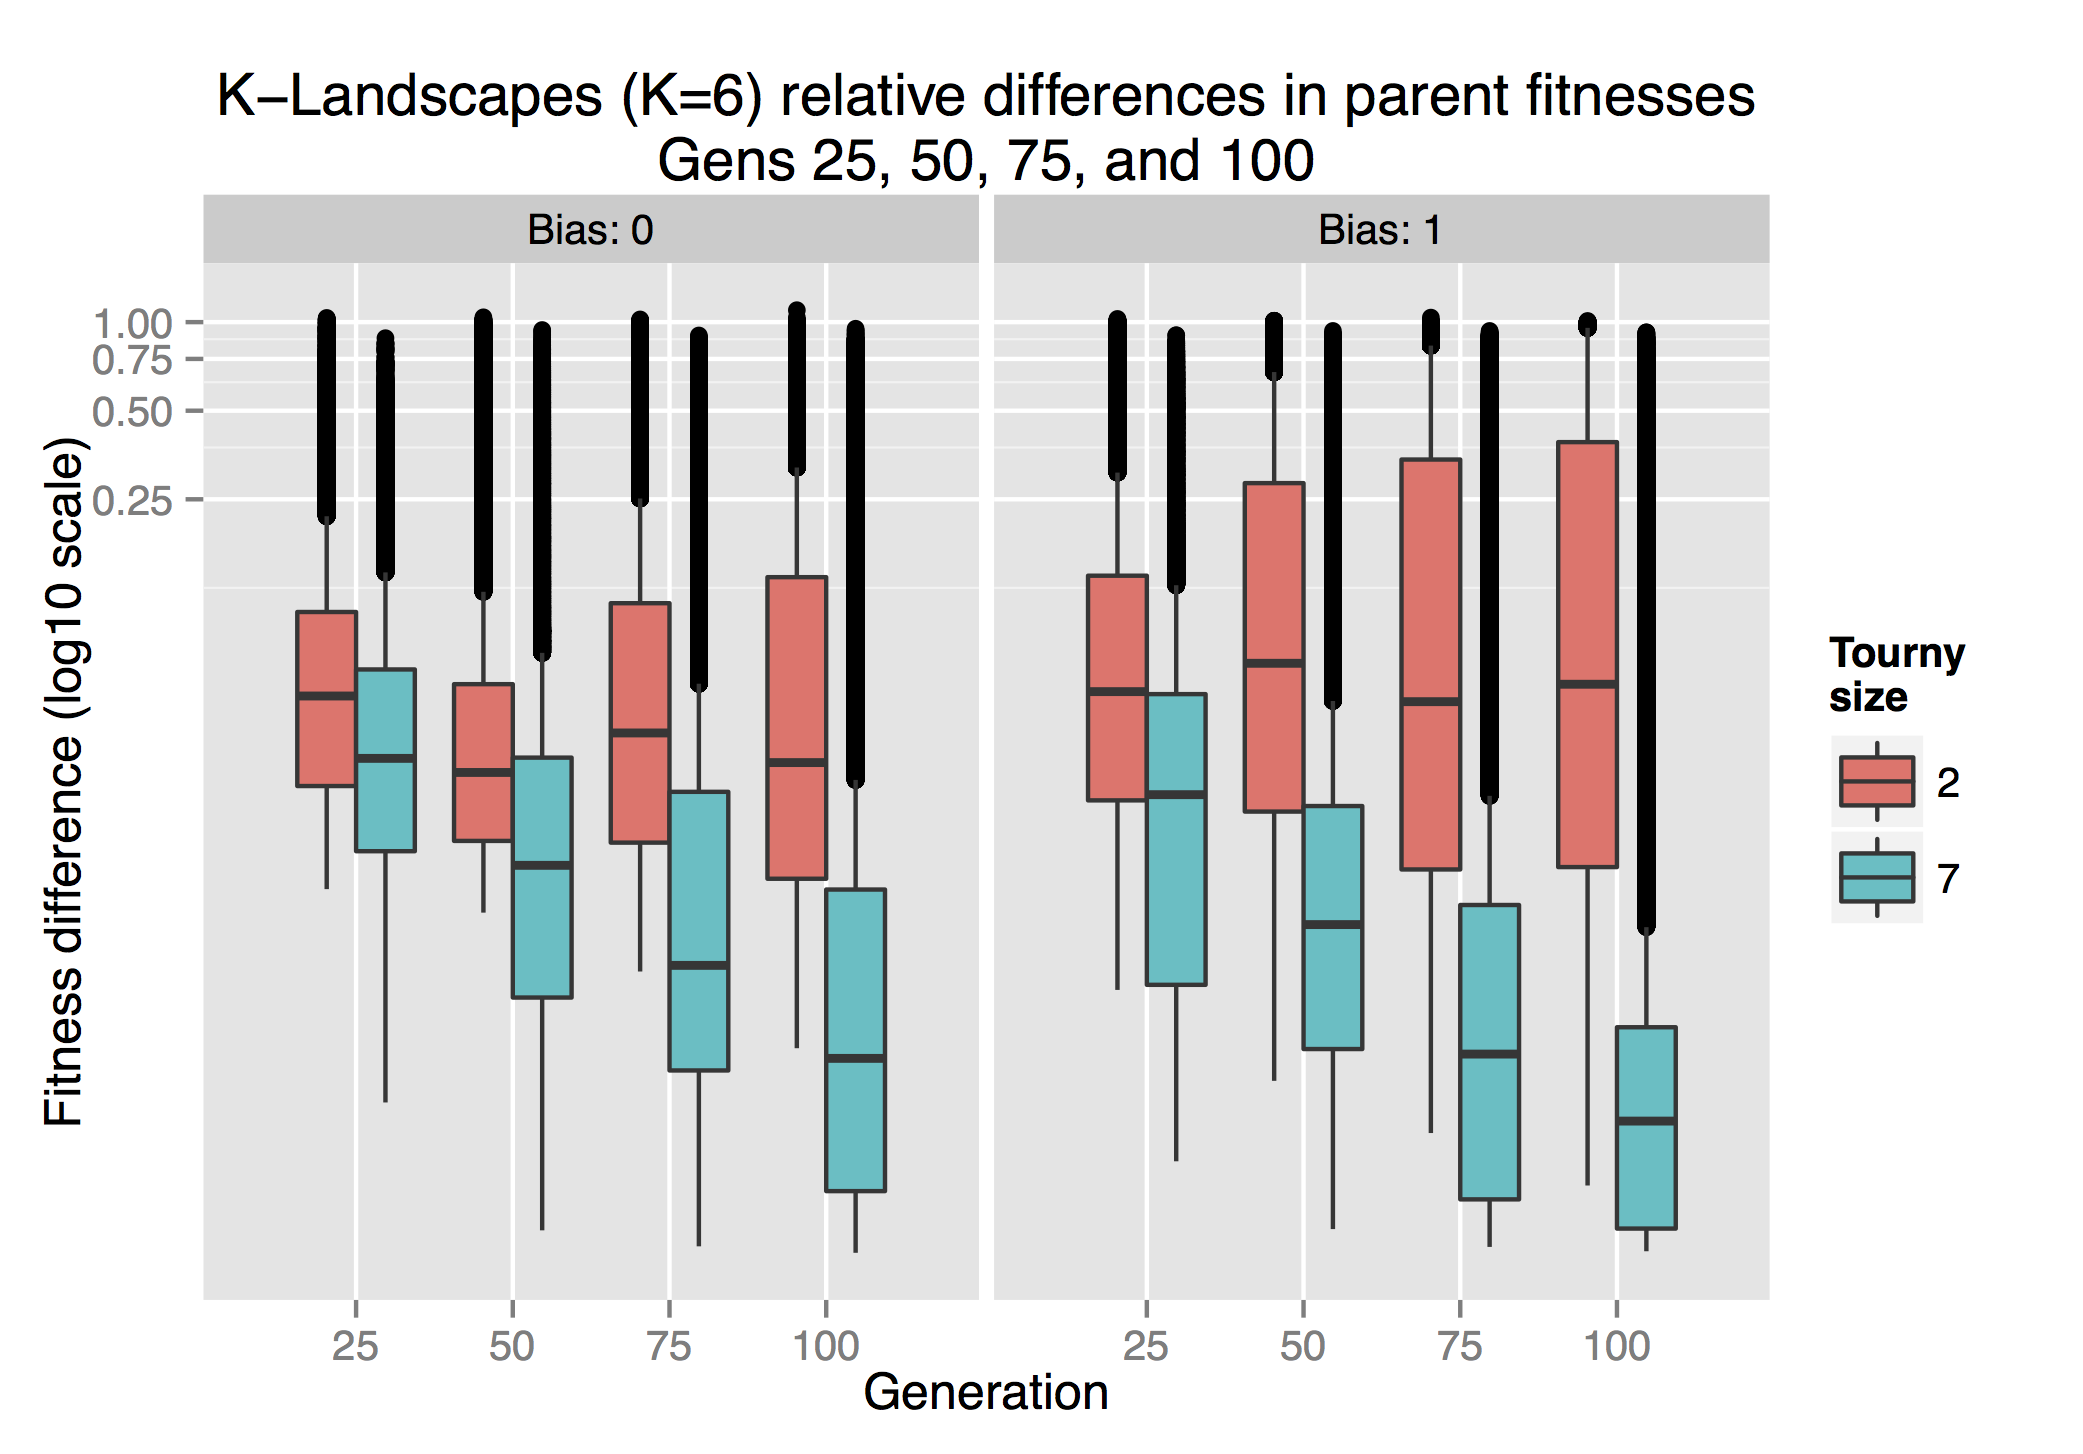
\includegraphics[width=0.45 \textwidth]{Plots/Parent_normalized_fitness_diffs_KLandscapes.pdf}
\caption{Plot of the normalized differences in parent fitnesses for the K Landscapes problem. The left-hand (and higher) boxplot in each pair of boxplots is for the binary tournament runs.}
\label{fig:parentDiffsKLandscapes}
\end{figure}

\begin{figure}[tb]
	\centering
	\includegraphics[width=0.45 \textwidth]{Plots/Parent_normalized_error_diffs_sine.pdf}
	\caption{Plot of the normalized differences in parent errors for the sine symbolic regression problem.  The left-hand (and higher) boxplot in each pair of boxplots is for the binary tournament runs.}
	\label{fig:parentDiffsSine}
\end{figure}

Our results also indicate that crossover bias may increase certain types of selection pressure, which could potentially
increase the likelihood of premature convergence.
% (see Figures~\ref{fig:sineBiasFitnessVsGenStrong} and~\ref{fig:sineBiasFitnessVsGenWeak}).
There is a heightened focus on the better of the two parents which increases the chance of the more fit parent's
semantics being carried across into the next generation. This might limit the diversity of the root structures causing
premature convergence. Further research is needed to understand if this does in fact lead to premature convergence in
some cases, but it's possible, for example, that this explains the fact that using some crossover bias (0.75) is better
than always using crossover bias in the ORDERTREE problem (see, e.g.,
Figure~\ref{fig:Ordertree_results_all_tournaments_Jan15}).

%In most of these experiments we found better results with tournament sizes of 7 than with binary tournaments, and in
%general using larger tournaments appears to wash out much of the impact of crossover bias, so there's a fair question
%about whether one should just use larger tournaments and ignore crossover bias. \textbf{How do we respond to this? I
%think the answer is something like ``It doesn't hurt (at least in our experiments), and it sometimes helps, even for
%tournament size 7 and with elitism. For interesting problems, you also don't know in advance what your best parameter
%choices are, so it's at least worth including in your arsenal.''}

\pagebreak 

\section{Conclusions} \label{sec:Conclusions}

Based on previous observations of interesting asymmetries in the behavior of sub-tree crossover
(e.g.,~\cite{McPheeDonatucciDramdahl:2014}), we introduced the idea of \emph{crossover bias}, where we
probabilistically force the more fit parent to be the \emph{root parent} when performing crossover. We then applied
this new bias to several different problems. In general, we found that adding crossover bias either
helps or is neutral, although there were cases where its effect was detrimental.

Given these results, it seems worthwhile to at least try crossover bias, especially in settings where there are reasons
to suspect that there are substantial differences between parental fitnesses. This is likely to be the case wherever
selection pressure is weak (e.g., our use of binary tournaments), but could also happen when there are unavoidable
steep changes in fitness, or in settings where the fitness function may vary over either time or as a function of some
other variable such as location.

A question to consider based on these results is whether or not we should use larger tournaments instead of crossover bias, since in many cases the results with tournament size 7 without crossover bias was as good or better than those obtained with binary tournaments and crossover bias, e.g., Figure~\ref{fig:KLandscapes6_XO_bias_impact_facets}. 
According to Gustafson et al.~\cite{Gustafson:2005}, however, matings between similar parents are more likely 
to produce no change in fitness, whereas a more diverse crossover increases the chances of offspring 
improving fitness. Larger tournaments are more likely to select two parents that are similar, at 
least in fitness, as seen in Figures~\ref{fig:parentDiffsKLandscapes} and~\ref{fig:parentDiffsSine};
an excellent illustration of this can be seen in Figure 2 in~\cite{Boetticher:2006}. Another attempt to find a balance of 
diversity between parents is called sexual selection, proposed by Goh et al.~\cite{gohsexualselection}. Their sexual selection
system mates individuals chosen at random (with no regard to fitness) with individuals chosen via tournament selection.
This creates a strong asymmetry between the parents which appears to increase diversity in certain circumstances in ways
that improve performance. Based on these examples, 
there may be circumstances where combining crossover bias with a weaker selection mechanism might be a reasonable alternative to using a larger tournament size. 

Another outstanding question is how crossover bias affects generalization, especially since it's possible that crossover
bias increases selection pressure and could consequently encourage overfitting. We didn't explore this question here, but
it would be useful to expand the existing work to include validation to see what impact, if any,
crossover bias has on how well evolved solutions generalize to unseen data.

While this paper focuses on asymmetry in the context of tree-based GP and sub-tree crossover, it's important to note
that asymmetries like this are common in many evolutionary systems, both biological and artificial. Much eukaryote
reproduction is sexual, and brings with it numerous sex-linked traits and related asymmetries; this may play an
important role in speciation~\cite{qvarnstrom2009speciation}, arguably one of the most crucial of biological
asymmetries. Many evolutionary computation systems other than tree-based GP also have significant asymmetries. Linear
GP systems~\cite{brameier2007linear} and stack-based GP systems~\cite{spector:2002:GPEM}, for example, have asymmetries
where the last instructions executed can have a disproportionate impact on the results. Similarly, changes near the
front of grammatical evolution~\cite{o2003grammatical} strings will have a disproportionate impact by determining the
important early choices in the grammar productions. Generally, these asymmetries weren't intentional, but
were instead simple artifacts of other system design decisions. Hence, the potential impact of these asymmetries has
been largely unstudied. The results presented here suggest that it may be important to more thoroughly explore the
impact of such asymmetries, both to better understand the performance and behavior of existing systems, but also as an
aid to the design and discovery of new tools like recombination operators that leverage these asymmetries.

 \section*{Acknowledgements}

 Many thanks to the members of the Hampshire College Computational Intelligence Lab for suggestions and feedback as
 this work developed, with particular thanks to Thomas Helmuth, William La Cava, and Lee Spector. Thanks also to Thomas
 Helmuth for introducing us to the U.S. Change problem. Thanks to W. B. Langdon and our anonymous reviewers 
 for valuable feedback and numerous suggestions. 
 
 David Donatucci's work was supported in part by a Morris Academic Partners grant from the Office for Academic Affairs and Dean at the University of Minnesota, Morris.

\bibliographystyle{abbrv}
\bibliography{Research_2015}

\end{document}